% Options for packages loaded elsewhere
\PassOptionsToPackage{unicode}{hyperref}
\PassOptionsToPackage{hyphens}{url}
%
\documentclass[
]{article}
\usepackage{amsmath,amssymb}
\usepackage{iftex}
\ifPDFTeX
  \usepackage[T1]{fontenc}
  \usepackage[utf8]{inputenc}
  \usepackage{textcomp} % provide euro and other symbols
\else % if luatex or xetex
  \usepackage{unicode-math} % this also loads fontspec
  \defaultfontfeatures{Scale=MatchLowercase}
  \defaultfontfeatures[\rmfamily]{Ligatures=TeX,Scale=1}
\fi
\usepackage{lmodern}
\ifPDFTeX\else
  % xetex/luatex font selection
\fi
% Use upquote if available, for straight quotes in verbatim environments
\IfFileExists{upquote.sty}{\usepackage{upquote}}{}
\IfFileExists{microtype.sty}{% use microtype if available
  \usepackage[]{microtype}
  \UseMicrotypeSet[protrusion]{basicmath} % disable protrusion for tt fonts
}{}
\makeatletter
\@ifundefined{KOMAClassName}{% if non-KOMA class
  \IfFileExists{parskip.sty}{%
    \usepackage{parskip}
  }{% else
    \setlength{\parindent}{0pt}
    \setlength{\parskip}{6pt plus 2pt minus 1pt}}
}{% if KOMA class
  \KOMAoptions{parskip=half}}
\makeatother
\usepackage{xcolor}
\usepackage{graphicx}
\makeatletter
\def\maxwidth{\ifdim\Gin@nat@width>\linewidth\linewidth\else\Gin@nat@width\fi}
\def\maxheight{\ifdim\Gin@nat@height>\textheight\textheight\else\Gin@nat@height\fi}
\makeatother
% Scale images if necessary, so that they will not overflow the page
% margins by default, and it is still possible to overwrite the defaults
% using explicit options in \includegraphics[width, height, ...]{}
\setkeys{Gin}{width=\maxwidth,height=\maxheight,keepaspectratio}
% Set default figure placement to htbp
\makeatletter
\def\fps@figure{htbp}
\makeatother
\setlength{\emergencystretch}{3em} % prevent overfull lines
\providecommand{\tightlist}{%
  \setlength{\itemsep}{0pt}\setlength{\parskip}{0pt}}
\setcounter{secnumdepth}{-\maxdimen} % remove section numbering
\ifLuaTeX
  \usepackage{selnolig}  % disable illegal ligatures
\fi
\IfFileExists{bookmark.sty}{\usepackage{bookmark}}{\usepackage{hyperref}}
\IfFileExists{xurl.sty}{\usepackage{xurl}}{} % add URL line breaks if available
\urlstyle{same}
\hypersetup{
  hidelinks,
  pdfcreator={LaTeX via pandoc}}

\author{}
\date{}

\begin{document}

\hypertarget{hidden-vortex-cores-and-false-confidence-in-measurement-resolution}{%
\section{Hidden vortex cores and false confidence in measurement
resolution}\label{hidden-vortex-cores-and-false-confidence-in-measurement-resolution}}

\hypertarget{exact-gaussian-filtering-conditional-certificates-and-a-reproducible-benchmark}{%
\subsection{Exact Gaussian filtering, conditional certificates, and a
reproducible
benchmark}\label{exact-gaussian-filtering-conditional-certificates-and-a-reproducible-benchmark}}

\textbf{Thomas Verdier}\\
Independent researcher, Charleston, South Carolina\\
Working research manuscript, version 0.3, 9 September 2026

\hypertarget{abstract}{%
\subsubsection{Abstract}\label{abstract}}

We analyze Gaussian measurements of a smooth, divergence-free vortex
whose spatial scales contract while its peak velocity increases. Exact
convolution yields a joint anisotropy-resolution crossover: reversing
two orders of limits changes the normalized maximum measured peak by
32/27. The true peak diverges while every fixed smooth observation
kernel with bounded derivatives produces a vanishing signal. Three
directional peak measurements yield deterministic scale and retention
intervals conditional on a single Gaussian profile. An explicit
two-component counterexample shows why this condition matters:
measurements consistent with approximately 98\% retention can represent
a flow retaining only 32.7\% of its actual peak. We also derive an
elementary, profile-independent necessary resolution bound from energy
and peak-growth estimates. Independent quadrature, high-precision
optimization checks, and 5,000 bounded-noise trials support the
calculations. Exploratory DNS pilots additionally show that conditional
model decisions can disagree with regional sampled peak ratios; profile
and field-of-view effects remain unresolved. These are results for a
kinematic benchmark, with a limited conditional application to reported
Navier-Stokes growth estimates; the Gaussian crossover is not
established for that complete flow.

\hypertarget{motivation-and-scope}{%
\subsubsection{1. Motivation and scope}\label{motivation-and-scope}}

OpenAI's September 2026 manuscript reports a forced, finite-energy
Navier-Stokes blowup construction. Its leading-core radial scale, axial
scale, and characteristic velocity scale are proportional to powers of
the time remaining before concentration: respectively tau\^{}(1/2),
tau\^{}(1/2-h), and tau\^{}(-1/2-h), with a small positive h {[}1,
Section 2{]}. These exponents motivate the benchmark below. We use them
as an explicit mathematical parameterization; none of our proofs assume
the validity of that construction.

The distinction between an unbounded continuum velocity and a bounded
measurement is elementary but consequential. For any velocity u in L2
and kernel K in L2, Cauchy-Schwarz gives

\[
\|K*u\|_\infty\leq \|K\|_2\|u\|_2. \tag{1}
\]

Consequently, a uniformly bounded-energy flow always has a bounded
filtered velocity at each fixed kernel width. Equation (1) does not
imply that its filtered signal vanishes or identify the resolution
needed to measure the peak.

Spatial filtering of measured vortices has substantial prior literature.
Rahgozar, Maciel and Schlatter study spatial-resolution effects on
vortex characterization in planar particle image velocimetry (PIV)
{[}2{]}. Deem and colleagues correct smoothing caused by vortex
wandering using deconvolution {[}3{]}. Gaussian scale selection has a
mature theory {[}4{]}, and the distinction between continuous and
discretized Gaussian operations is quantitatively important {[}5{]}.
Numerical investigations of fluid singularities also depend on the
interaction of geometric scales, computation, and analysis {[}6{]}.
Recent learned reconstructions of PIV vortex flows provide another
comparison point {[}7{]}.

The closest analytic comparison is Lindeberg's treatment of anisotropic
Gaussian blobs and exact extrema over scale {[}8, Sections 3.3 and
5.2{]}. Accordingly, Gaussian closure, anisotropic scale optimization,
width recovery, and deconvolution instability are not claimed as new.
The narrower contribution is the explicit joint limit along the selected
concentration path, accompanied by reproducible conditional diagnostics
and a hidden-core counterexample. The observables differ: {[}8{]}
studies image differential responses, while here we maximize filtered
vector speed over space and concentration time. A targeted search found
no exact prior instance of the 32/27 result; this does not establish
priority. We position the work as a methods and benchmark note.

\textbf{Scope.} This is an observation-theory benchmark. It is not a
solution of the forced Navier-Stokes problem, an implementation of the
oscillatory corrections in {[}1{]}, or a model of an entire PIV
acquisition pipeline. Filter widths denote Gaussian standard deviations,
not mesh spacings. All spatial norms below use the Euclidean vector
norm, and spatial peaks are continuum suprema. Discrete sampling error
is an additional measurement error.

\hypertarget{an-explicit-solenoidal-concentration-family}{%
\subsubsection{2. An explicit solenoidal concentration
family}\label{an-explicit-solenoidal-concentration-family}}

Let a,b,U be positive. With x=(x1,x2,z), define

\[
\phi_{a,b}(x)=\exp\!\left(-\frac{x_1^2+x_2^2}{2a^2}-\frac{z^2}{2b^2}\right),
\qquad
u_{a,b,U}(x)=\frac{\sqrt{e}\,U}{a}(-x_2,x_1,0)\phi_{a,b}(x). \tag{2}
\]

For tau\textgreater0 and 0\textless=h\textless0.01, set

\[
a=\tau^{1/2},\qquad b=\tau^{1/2-h},\qquad U=\tau^{-1/2-h}. \tag{3}
\]

The endpoint h=0 is an isotropic comparison family. Each field is
smooth, rapidly decreasing and divergence-free. Its flow direction is
purely azimuthal. In particular, it does not reproduce radial inflow,
axial stretching, or the nonlinear stress corrections of {[}1{]}.

\textbf{Proposition 1 (peak and energy).} The family (2) satisfies

\[
\nabla\cdot u=0,\qquad \|u\|_\infty=U,\qquad
E:=\frac12\int_{\mathbb R^3}|u|^2\,dx
=\frac{e\pi^{3/2}}2 U^2a^2b. \tag{4}
\]

Under (3), E=(e*pi\^{}(3/2)/2) tau\^{}(1/2-3h), whereas the peak is
tau\^{}(-1/2-h).

\emph{Proof.} The derivatives of the two nonzero components cancel in
the divergence. At fixed z, the speed is proportional to r
exp(-r\textsuperscript{2/(2a}2)), with maximum at r=a; the maximum in z
occurs at zero. The factor sqrt(e) makes this peak exactly U. In
cylindrical coordinates, integration uses int\_0\^{}infinity r\^{}3
exp(-r\textsuperscript{2/a}2) dr=a\^{}4/2 and int\_R
exp(-z\textsuperscript{2/b}2) dz=sqrt(pi)b. This gives (4). Substitution
of (3) gives the exponents. QED.

\textbf{Dynamical distinction.} The prescribed family cannot be
maintained by a force smooth through tau=0. Set t=1-tau and viscosity
nu\textgreater0. At r=a,z=0, its azimuthal momentum balance requires the
angular mean of the azimuthal force to be

\[
\langle f_\theta\rangle_\theta
=U\left[\frac{1/2+h+3\nu}{\tau}+\nu\tau^{-1+2h}\right]. \tag{4a}
\]

Indeed, the azimuthal material derivative here is partial\_t
u\_theta=(1/2+h)U/tau, and the azimuthal component of the vector
Laplacian is -(3/a\textsuperscript{2+1/b}2)U. The angular average of an
azimuthal pressure derivative is zero. Expression (4a) diverges at
points approaching the origin. This verifies that the benchmark studies
observation effects separately from smooth-force Navier-Stokes dynamics.

\hypertarget{fixed-kernel-disappearance-and-a-noise-obstruction}{%
\subsubsection{3. Fixed-kernel disappearance and a noise
obstruction}\label{fixed-kernel-disappearance-and-a-noise-obstruction}}

Write grad\_perp K=(partial\_2 K,-partial\_1 K,0), and let
C0=sqrt(e)(2pi)\^{}(3/2). For a scalar kernel K with bounded derivatives
through order three, define H\_K as the supremum of the bilinear
operator norm of D\^{}2 grad\_perp K.

\textbf{Theorem 2 (a dipole observation limit).} If K is integrable, C3,
and has bounded derivatives through order three, then

\[
\|K*u-C_0Ua^3b\,\nabla_\perp K\|_\infty
\leq \frac{C_0}{2}Ua^3b(2a^2+b^2)H_K. \tag{5}
\]

If grad\_perp K is nonzero and a,b tend to zero, then

\[
\|K*u\|_\infty\sim C_0Ua^3b\|\nabla_\perp K\|_\infty. \tag{6}
\]

For (3), Ua\textsuperscript{3b=tau}(3/2-2h); hence the filtered signal
vanishes uniformly while the true peak diverges.

\emph{Proof.} From (2), u=sqrt(e)Ua grad\_perp phi. Moving the
derivative onto K by integration by parts yields K*u=C0Ua\^{}3b
E{[}grad\_perp K(x-Y){]}, where Y is centered Gaussian with covariance
diag(a\textsuperscript{2,a}2,b\^{}2). Taylor-expand grad\_perp K at x.
The first-order term has zero expectation. The vector remainder is
bounded by H\_K \textbar Y\textbar\^{}2/2, whose expectation is
H\_K(2a\textsuperscript{2+b}2)/2. This proves (5). The reverse triangle
inequality for the supremum norm proves (6). QED.

The additional factor a in Ua\^{}3b reflects cancellation of oppositely
directed velocities across the vortex. Filtering the vector velocity and
then taking its magnitude differs from filtering the scalar speed. All
results here use the former observation convention.

\textbf{Corollary 3 (bounded-noise indistinguishability).} Consider any
finite collection of fixed kernels satisfying Theorem 2. Suppose each
complete filtered velocity field is observed with additive error bounded
by sigma\textgreater0 in the supremum norm. For all sufficiently small
tau, there is an observation compatible both with u\_tau and with the
zero field. Any peak estimator based only on that snapshot has
worst-case absolute error at least U(tau)/2 over these two
possibilities.

\emph{Proof.} For small tau all filtered norms are at most 2sigma. The
collection of half-signals y\_j=(K\_j*u\_tau)/2 is within sigma of both
the zero observation and the signal. An estimate p based on this common
observation must satisfy
max(\textbar p\textbar,\textbar p-U\textbar)\textgreater=U/2. QED.

This is a noise-stability obstruction, not a failure of injectivity for
noiseless Gaussian convolution. It assumes snapshot data and does not
exclude inferences using additional dynamics, a known trajectory, or
restrictive prior information.

\hypertarget{exact-gaussian-measurements-and-apparent-decay}{%
\subsubsection{4. Exact Gaussian measurements and apparent
decay}\label{exact-gaussian-measurements-and-apparent-decay}}

Let d and eta be positive radial and axial observation widths. Define
the normalized Gaussian

\[
G_{d,\eta}(x)=\frac{\exp[-(x_1^2+x_2^2)/(2d^2)-z^2/(2\eta^2)]}
{(2\pi)^{3/2}d^2\eta}. \tag{7}
\]

\textbf{Theorem 4 (exact transfer function).} Put
A=sqrt(a\textsuperscript{2+d}2), B=sqrt(b\textsuperscript{2+eta}2). Then
G*u is exactly the field (2) with parameters A,B,M, where

\[
M=U\left(1+\frac{d^2}{a^2}\right)^{-3/2}
\left(1+\frac{\eta^2}{b^2}\right)^{-1/2}. \tag{8}
\]

\emph{Proof.} Gaussian convolution gives
G*phi=(a\textsuperscript{2b/(A}2B))exp{[}-r\textsuperscript{2/(2A}2)-z\textsuperscript{2/(2B}2){]}.
Applying sqrt(e)Ua grad\_perp yields
sqrt(e)Ua\textsuperscript{3b(-x2,x1,0)exp{[}-r\textsuperscript{2/(2A}2)-z\textsuperscript{2/(2B}2){]}/(A}4B).
Its speed is maximal at r=A,z=0, proving (8). QED.

For fixed d,eta and (3), the late-concentration asymptotic is

\[
M\sim d^{-3}\eta^{-1}\tau^{3/2-2h}. \tag{9}
\]

For a more general family a=tau\^{}alpha, b=tau\^{}beta,
U=tau\^{}(-gamma), differentiating (8) gives

\[
\frac{d\log M}{d\log\tau}=-\gamma+
\frac{3\alpha d^2}{\tau^{2\alpha}+d^2}+
\frac{\beta\eta^2}{\tau^{2\beta}+\eta^2}. \tag{10}
\]

When alpha,beta,gamma\textgreater0 and gamma\textless3alpha+beta, the
right side strictly decreases with tau from a positive value to a
negative one. Thus M has exactly one maximum on tau\textgreater0. As
concentration proceeds toward tau=0, the measured peak first rises and
then falls, despite continuing growth of U. A physical time interval
such as 0\textless tau\textless=1 contains this maximum when the
observation widths are sufficiently small.

\hypertarget{a-singular-anisotropy-resolution-crossover}{%
\subsubsection{5. A singular anisotropy-resolution
crossover}\label{a-singular-anisotropy-resolution-crossover}}

We now take d=eta=delta and use (3). Let M\_h(tau,delta) denote (8), and
define

\[
P_h(\delta)=\delta^{1+2h}\sup_{\tau>0}M_h(\tau,\delta). \tag{11}
\]

\textbf{Theorem 5 (noncommuting limits).} The two iterated limits exist
and satisfy

\[
\lim_{h\downarrow0}\lim_{\delta\downarrow0}P_h(\delta)
=\frac{2}{3\sqrt3},\qquad
\lim_{\delta\downarrow0}\lim_{h\downarrow0}P_h(\delta)
=\frac{3\sqrt3}{16}. \tag{12}
\]

Their ratio is 32/27, or approximately 1.185185. More precisely, if h
and delta tend to zero with h log(1/delta) tending to chi\textgreater=0,
then

\[
P_h(\delta)\longrightarrow C(\chi)
=\frac{s_*^{3/2}}{(s_*+1)^{3/2}(s_*+e^{-4\chi})^{1/2}},
\qquad s_*=1+\sqrt{1+3e^{-4\chi}}. \tag{13}
\]

The maximizing concentration time obeys tau\_peak/delta\^{}2
-\textgreater{} s\_* in this joint limit.

\emph{Proof.} Set tau=delta\^{}2 s and chi=h log(1/delta). The
normalized response is exactly

\[
F_{h,\chi}(s)=s^{-1/2-h}(1+s^{-1})^{-3/2}
(1+e^{-4\chi}s^{-1+2h})^{-1/2}. \tag{14}
\]

For h tending to zero and chi tending to a fixed nonnegative value, (14)
converges locally uniformly on s\textgreater0 to

\[
F_\chi(s)=\frac{s^{3/2}}{(s+1)^{3/2}(s+e^{-4\chi})^{1/2}}. \tag{15}
\]

The convergence passes to maxima: for 0\textless s\textless=1 and
0\textless=h\textless=h0\textless0.01, F is at most s\^{}(1-h0); for
s\textgreater=1 it is at most s\^{}(-1/2). These bounds make both tails
uniformly negligible. Differentiating log(F\_chi\^{}2) gives
3/s-3/(s+1)-1/(s+exp(-4chi)); its unique zero is s\_* in (13).
Uniqueness and local uniform convergence also give convergence of
maximizers.

For fixed h\textgreater0, sending delta to zero in (14) removes its last
factor. The limiting maximum occurs at c\_h=3/(1+2h)-1, and has value

\[
c_h^{-1/2-h}\left(\frac{c_h}{1+c_h}\right)^{3/2}. \tag{16}
\]

Sending h to zero gives 2/(3sqrt(3)). In the reverse order, h=0 gives
F=s\textsuperscript{(3/2)/(s+1)}2, whose maximum is at s=3 and equals
3sqrt(3)/16. This proves (12). QED.

For 0\textless tau\textless=1 the same small-delta limits apply, because
the maximizing tau is of order delta\^{}2. The crossover can be
extremely slow: the factor controlling it is delta\^{}(4h), so small
positive anisotropy cannot generally be treated as either fully
isotropic or fully separated at accessible resolutions. The factor 32/27
describes the normalized maximum over concentration time, not the
instantaneous attenuation at a fixed time.

\hypertarget{a-resolution-certificate-from-three-observations}{%
\subsubsection{6. A resolution certificate from three
observations}\label{a-resolution-certificate-from-three-observations}}

Assume that the isolated vortex component is described by (2), with
unknown positive a,b,U but known observation widths. Let M0 be the peak
at widths (d,eta), Mr the peak at (kappa\emph{d,eta), and Mz the peak at
(d,kappa}eta), where kappa\textgreater1. Define

\[
Q_r=(M_0/M_r)^{2/3},\qquad Q_z=(M_0/M_z)^2.
\tag{17}
\]

\textbf{Proposition 6 (exact scale recovery).} The scale parameters
satisfy

\[
a^2=d^2\frac{\kappa^2-Q_r}{Q_r-1},\qquad
b^2=\eta^2\frac{\kappa^2-Q_z}{Q_z-1},\qquad 1<Q_r,Q_z<\kappa^2. \tag{18}
\]

The amplitude then follows from (8). This requires no value for tau or
h.

\emph{Proof.} Ratios cancel U and the unchanged directional attenuation.
Raising to the exponents in (17) leaves (a\textsuperscript{2+kappa}2
d\textsuperscript{2)/(a}2+d\^{}2), and the analogous expression for b.
Rearranging gives (18). QED.

The coarser fields can be produced by additionally smoothing the base
field with radial or axial standard deviation sqrt(kappa\^{}2-1) times
the base width. This operation does not restore information lost in the
base observation. The inversion uses the assumed family; it becomes
ill-conditioned as Q approaches either endpoint.

\textbf{Deterministic error intervals.} Let the observed base and
coarser peaks be m0,m1, with known absolute errors eps0,eps1. If both
observed peaks exceed their respective errors, then the true ratio
belongs to

\[
\left[\frac{m_0-\epsilon_0}{m_1+\epsilon_1},
\frac{m_0+\epsilon_0}{m_1-\epsilon_1}\right]. \tag{19}
\]

Raise both endpoints to 2/3 for a radial comparison or 2 for an axial
comparison. Intersect with the admissible interval (1,kappa\^{}2), then
map through the decreasing function F\_w(Q)=w
sqrt((kappa\^{}2-Q)/(Q-1)). Reversing the endpoints gives a rigorous
radius enclosure. An interval touching Q=kappa\^{}2 has lower radius
bound zero; one touching Q=1 has upper bound infinity. If a denominator
cannot be separated from zero, return {[}0,infinity{]}. An empty
admissible intersection reports inconsistency with the model and stated
error bounds.

Let {[}aL,aH{]} and {[}bL,bH{]} be the resulting enclosures, and define

\[
R(a,b)=(1+d^2/a^2)^{-3/2}(1+\eta^2/b^2)^{-1/2}. \tag{20}
\]

Because R increases in both arguments, a target retention rho is
certified if R(aL,bL)\textgreater=rho. Underresolution is certified if
R(aH,bH)\textless rho. Otherwise the result is indeterminate. The
conventions are R=0 if either size is zero, and w\^{}2/infinity=0. These
are conservative statements conditional on the vortex model and valid
error bounds.

\textbf{Arithmetic and scope.} Ordinary floating-point evaluation need
not enclose exact endpoints, even with zero measurement error. For
example, the radial inputs m0=27, m1=8, d=1, kappa=2 give a=sqrt(7/5); a
collapsed interval at its rounded value misses that exact radius. The
revised implementation treats supplied numbers as exact rational inputs,
encloses radial cube roots by rational bisection, and verifies
outward-rounded radius endpoints by exact squared comparisons. Retention
decisions also use exact rational squared comparisons. This establishes
conservative arithmetic enclosures for the supplied inputs; upstream
computation and measurement errors must still be included. Three peaks
determine three model parameters and cannot independently validate the
profile or exclude an unresolved component.

\hypertarget{model-error-and-transfer-to-a-complete-flow}{%
\subsubsection{7. Model error and transfer to a complete
flow}\label{model-error-and-transfer-to-a-complete-flow}}

Suppose the observed flow is u+w. For each Gaussian filter,

\[
\big|\|G*(u+w)\|_\infty-\|G*u\|_\infty\big|
\leq\|G*w\|_\infty\leq
\frac{\|w\|_2}{\sqrt{8\pi^{3/2}d^2\eta}}. \tag{21}
\]

Thus a proved L2 bound on w can be added to the observation-error budget
after multiplication by the explicit factor in (21). The ensuing
certificate concerns the modeled component u; it is not automatically a
certificate for the total flow's peak.

Relative smallness in energy is insufficient to preserve the leading
measured signal. Let v be a fixed, nonzero smooth Gaussian vortex and
w\_tau=tau*v. Under (3),

\[
\frac{\|w_\tau\|_2}{\|u_\tau\|_2}\asymp\tau^{3/4+3h/2}\to0,
\qquad
\frac{\|G*w_\tau\|_\infty}{\|G*u_\tau\|_\infty}
\asymp\tau^{-1/2+2h}\to\infty. \tag{22}
\]

This follows directly from Proposition 1, Theorem 2, and linearity of
filtering. A correction negligible relative to the core's L2 norm can
dominate its fixed-resolution observation. To carry (9) over to a
complete construction, one needs direct filtered-error control,
cancellation estimates, or the sufficient condition
\textbar\textbar w\textbar\textbar2=o(Ua\^{}3b) at fixed widths. A
regular exterior background must also be accounted for. The complete
solution may have a nonzero filtered background even when an isolated
concentrating component disappears.

\textbf{Proposition 7 (a necessary resolution bound without a profile
assumption).} Suppose a velocity family v\_tau satisfies
\textbar\textbar v\_tau\textbar\textbar2\textless=B and
\textbar\textbar v\_tau\textbar\textbar infinity\textgreater=c
tau\^{}(-gamma), where B,c,gamma are positive constants. If a Gaussian
observation retains a fraction at least rho of the actual peak, with
0\textless rho\textless1, then

\[
d^2\eta\leq\frac{B^2\tau^{2\gamma}}{8\pi^{3/2}\rho^2c^2}.
\tag{23}
\]

For isotropic width delta, this requires delta\textless=C
tau\^{}(2gamma/3), where C is the cube root of
B\textsuperscript{2/(8pi}(3/2)rho\textsuperscript{2c}2). At fixed
widths, the actual retained fraction is at most B tau\^{}gamma/(c
sqrt(8pi\textsuperscript{(3/2)d}2 eta)), and hence tends to zero.

\emph{Proof.} Direct integration gives
\textbar\textbar G\textbar\textbar2=(8pi\textsuperscript{(3/2)d}2
eta)\^{}(-1/2). The retention assumption and (1) imply rho c
tau\^{}(-gamma)\textless=rho
\textbar\textbar v\_tau\textbar\textbar infinity\textless=\textbar\textbar G*v\_tau\textbar\textbar infinity\textless=B\textbar\textbar G\textbar\textbar2.
Squaring and rearranging yields (23). Dropping the retention assumption
and dividing (1) by the peak lower bound gives the last assertion. QED.

This is an elementary consequence of an established energy inequality.
It is necessary, generally not sharp, and gives no sufficient sampling
rule or absolute disappearance result.

\textbf{What transfers to {[}1{]}.} Theorem 3.1(iv), equation (3.6), and
the localized growth path (10.21) give the required peak lower bound
with gamma=1/2+h and c=e0/2 at sufficiently small tau. Lemma 10.4
permits B=F(1). Conditional on those results, (23) therefore requires
delta\textless=C tau\^{}((1+2h)/3). Their pointwise growth estimate does
not supply our Gaussian observation law. Their profiles, exterior field,
and corrections differ, and their fixed-parameter bounds do not provide
the h-uniform control needed for Theorem 5 {[}1, Sections 3.1 and
3.6{]}. Thus (23), rather than 32/27 or (9), is the justified connection
to the complete flow.

\textbf{A hidden-core counterexample.} Add two concentric, co-rotating
copies of (2): a broad component with (a,b,U)=(10,10,1) and a narrow
component with (a,b,U)=(0.01,0.01,3). Take filter widths (1,1), (2,1),
and (1,2). The narrow component's L2 norm is only 9.49e-5 times the
broad component's, yet it controls the true peak. Denoting the total
field by v, alignment at the narrow core and the triangle inequality
give

\[
\frac{\|G_{1,1}*v\|_\infty}{\|v\|_\infty}
\leq\frac{(1+0.01)^{-2}+3(1+10000)^{-2}}{3}
<0.327. \tag{24}
\]

This conclusion requires no numerical maximization. Each filtered
narrow-core peak is below 3e-8. Therefore the broad component's three
peaks, with absolute error bound 4e-8, are compatible with either the
broad field alone or the total field. Those same data yield a
single-profile retention interval {[}0.98029599,0.98029611{]} and a
positive 90\% certificate. It is valid for the broad component and
invalid if interpreted as a certificate for the total peak. Tiny
measurement errors and tiny relative L2 profile errors do not resolve
this ambiguity.

Direct numerical maximization gives a total true peak of 3.001648947, a
base filtered peak of 0.9802960494, and actual retention of
0.3265858422. Using all three numerically maximized peaks with error
bounds 1e-12 also returns approximately 98\% model retention. Equation
(24) and the common-observation argument establish the failure
independently of the precision of that optimizer.

\begin{figure}
\centering
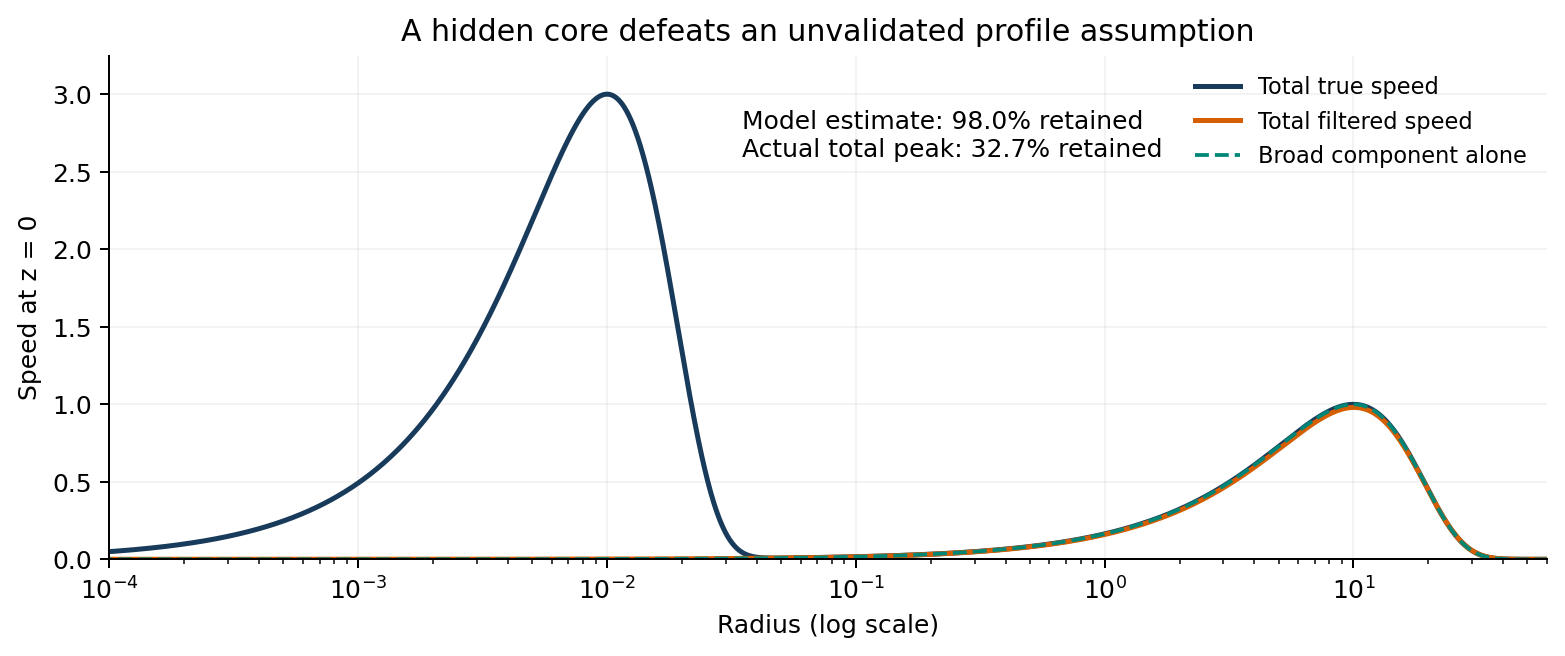
\includegraphics{figures/04_hidden_core.png}
\caption{Two concentric components: the broad vortex determines the
filtered signal while a narrow core determines the true peak. The
certificate remains conditional on the profile assumption.}
\end{figure}

\hypertarget{reproducible-computations}{%
\subsubsection{8. Reproducible
computations}\label{reproducible-computations}}

The script \texttt{reproduce.py} evaluates the closed forms and performs
independent numerical cross-checks; \texttt{review\_audit.py} adds
high-precision, boundary, and hidden-core checks. All generated data are
in \texttt{data/}, and figures are in \texttt{figures/}. Calculations
used Python 3.12.13, NumPy 2.3.5, SciPy 1.17.0, and Matplotlib 3.10.8.
The random seed is 20260909. These synthetic checks involve no PDE
integration or trained reconstruction model. A separate external DNS
pilot is described below.

\textbf{Convolution checks.} Forty randomly parameterized evaluations
used adaptive quadrature of the convolution integrals in source
coordinates, truncated at twelve Gaussian standard deviations. The
maximum vector error normalized by the exact peak was 9.87e-16. A second
check filtered a sampled velocity component on 49\^{}3, 65\^{}3, 97\^{}3
and 129\^{}3 grids. The central-line values agreed with the continuum
formula to less than 1.1e-15 of its peak. The finite grid still
underestimated the continuum line peak by 1.62\%, 0.850\%, 0.0431\% and
0.0245\%, respectively. Agreement of convolution values therefore does
not remove peak-sampling error. These are floating-point checks, not
interval-arithmetic certificates.

\textbf{Concentration trajectory.} With h=0.005 and d=eta=0.02, tau
ranged from 1 to 1e-14 on 1,001 logarithmically spaced points. The
measured peak reached approximately 16.9346 at the sampled
tau=0.00114815. At the final point the true peak was approximately
1.175e7, the measured peak 8.63e-15, and kinetic energy 1.62e-7 of its
initial value. A fit on tau\textless1e-10 gave a measured decay exponent
of 1.48999997, compared with the analytic 1.49.

\begin{figure}
\centering
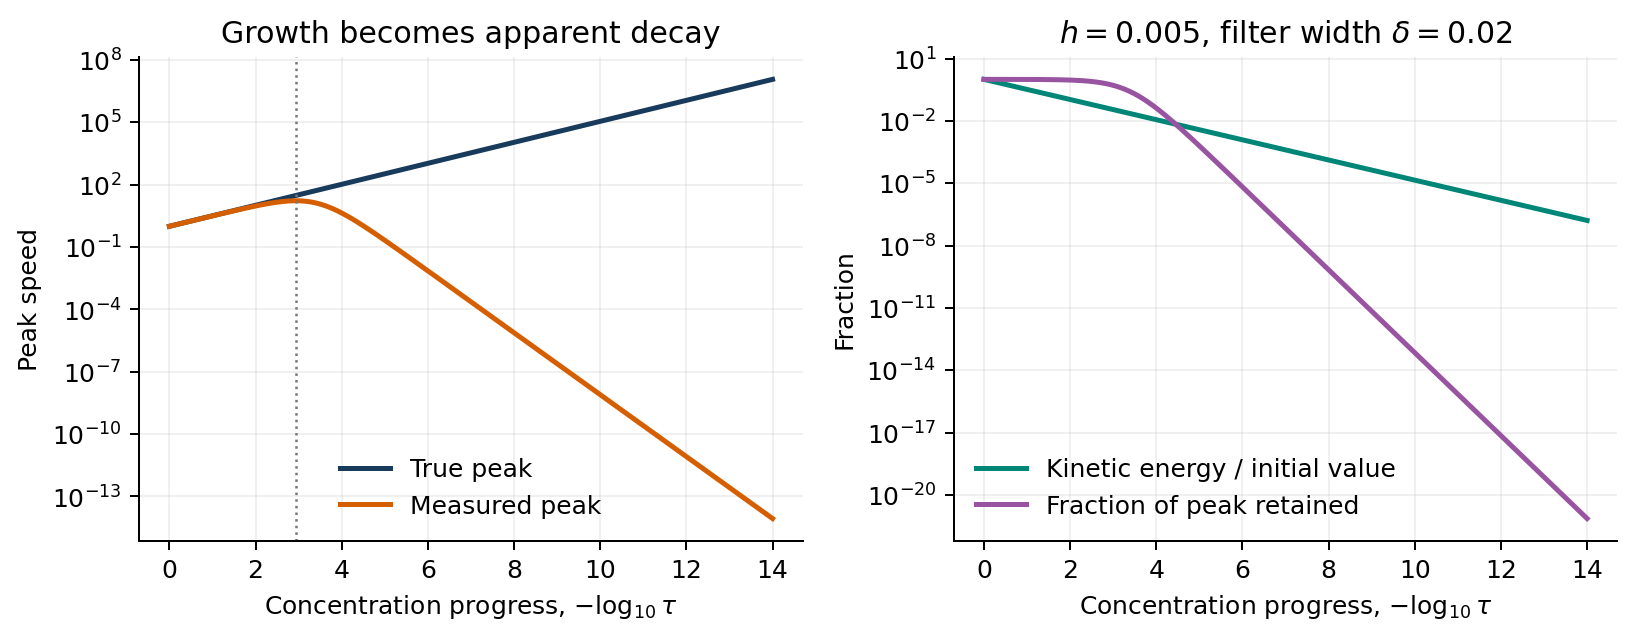
\includegraphics{figures/01_apparent_decay.png}
\caption{True peak, measured peak, and energy along the concentration
family.}
\end{figure}

\textbf{Crossover.} Numerical optimization of the exact normalized
response (14), on 101 values of chi from 0 to 2, was compared with (13).
Maximum relative differences in the normalized peak were 1.218\%,
0.681\%, and 0.137\% for h=0.009, 0.005, and 0.001. These differences
are finite-h effects. The analytic iterated-limit values are
0.3247595264 and 0.3849001795.

\begin{figure}
\centering
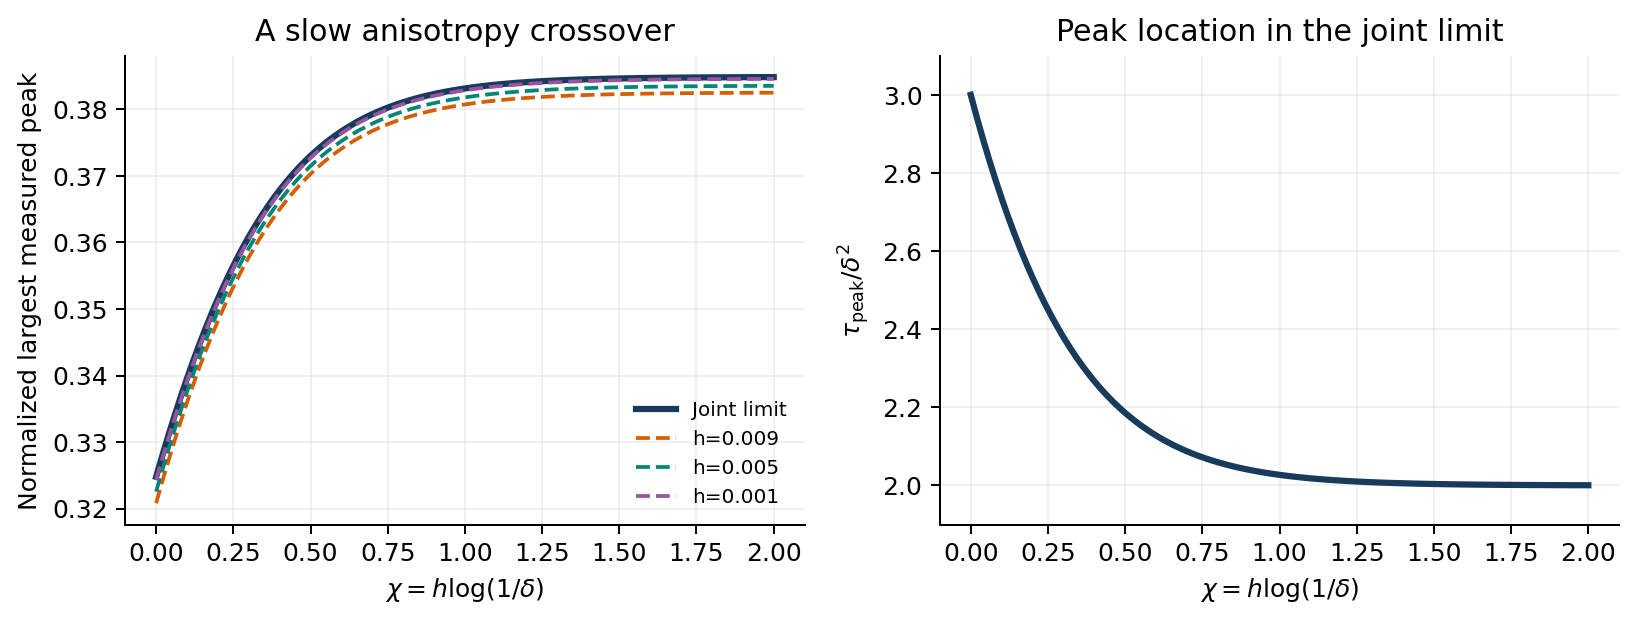
\includegraphics{figures/02_crossover.png}
\caption{The anisotropy-resolution crossover and the normalized peak
time.}
\end{figure}

\textbf{Independent maximum audit.} An 80-digit Decimal implementation
bisected the stationary equation directly in 24 cases: h in
\{0,0.001,0.005,0.009\} and chi in \{0,0.1,0.5,1,5,20\}. Its peak values
agreed with the SciPy optimizer to relative error at most 2.23e-16; the
maximizing locations agreed within 4.0e-8 relative error. The h=0 cases
also matched the closed-form crossover. These checks use different
numerical methods but do not replace the proof of the joint limit.

\textbf{Bounded-noise certificate.} In 5,000 trials, a and b were
independently log-uniform on {[}10\textsuperscript{(-1.5),10}(1.5){]},
U=1, d=eta=1, and kappa=2. Each of the three exact peaks received an
independent uniform perturbation in {[}-1e-4,1e-4{]}; that same absolute
bound was passed to the interval algorithm. For a 90\% retention target,
3,507 cases were certified underresolved, 525 resolved, and 968
indeterminate. All true sizes were enclosed. There were zero false
resolved and zero false underresolved decisions. Zero observed failures
are a verification result on these synthetic trials; deterministic
validity follows from (19) under its assumptions.

\begin{figure}
\centering
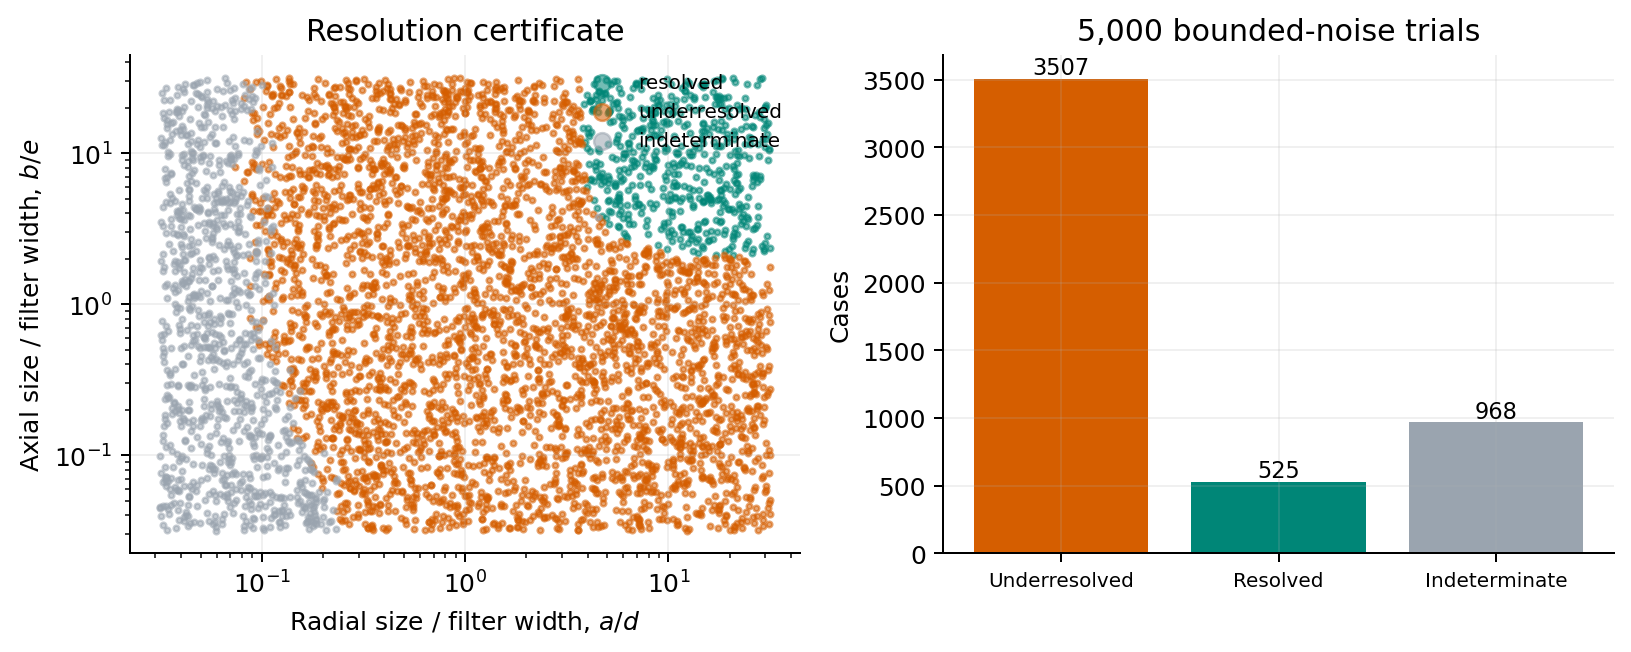
\includegraphics{figures/03_certification.png}
\caption{Certified resolution decisions under bounded additive noise.}
\end{figure}

\textbf{Boundary and arithmetic audit.} The revised enclosure algorithm
passed two exact rational square-root tests, seven endpoint/noise cases,
four invalid-input checks, and all eight noise corners on 28 shape pairs
(224 cases), including nearly saturated ratios. The corner checks used
80-digit reference peaks and budgets including float-conversion error.
All known radii and retentions were enclosed. The original 5,000 trials
were rerun after the arithmetic repair with unchanged decision counts.
The new hidden-core example is an intentional out-of-model failure, not
one of those in-model trials.

The trials test algebra, implementation, and conservative abstention
under the stated family. They do not measure performance on a turbulent
flow, compare with modern PIV reconstruction methods, or establish
robustness to unknown profile shape. Noise bounds on experimentally
inferred peaks must incorporate interpolation, calibration, filtering,
finite field of view, and background subtraction errors where relevant.

\textbf{External DNS pilot.} Eight separated 15\^{}3 cutouts from JHTDB
isotropic1024coarse {[}9{]}, at time index 1, were processed in two
frame conventions and at three base widths (0.35, 0.5, and 0.7 native
grid spacings). All peaks were evaluated on the same central 3\^{}3 grid
region with sufficient halo for the finite filter support. Among 48
correlated assessments, the conditional algorithm returned 38 resolved,
one underresolved, and nine model-inconsistent outputs. No resolved
output had a regional sampled peak ratio below 0.9. Ratios ranged from
0.88863 to 1.01820; a regional ratio can exceed one when filtering
imports a larger surrounding velocity. These ratios are not global
continuum peak retentions.

The pilot exercises the code on an external dataset but does not
validate the profile assumption, establish an error bound, or estimate
hidden-core prevalence. Its tolerance of 1e-4 times the regional
reference peak is a diagnostic setting. The small widths and evaluation
region limit what the negative result can show. Full acquisition
provenance, definitions, and a prospective study protocol accompany the
release in \texttt{EXTERNAL\_VALIDATION.md}, \texttt{DATA\_SOURCES.md},
and \texttt{STUDY\_PROTOCOL.md}.

\begin{figure}
\centering
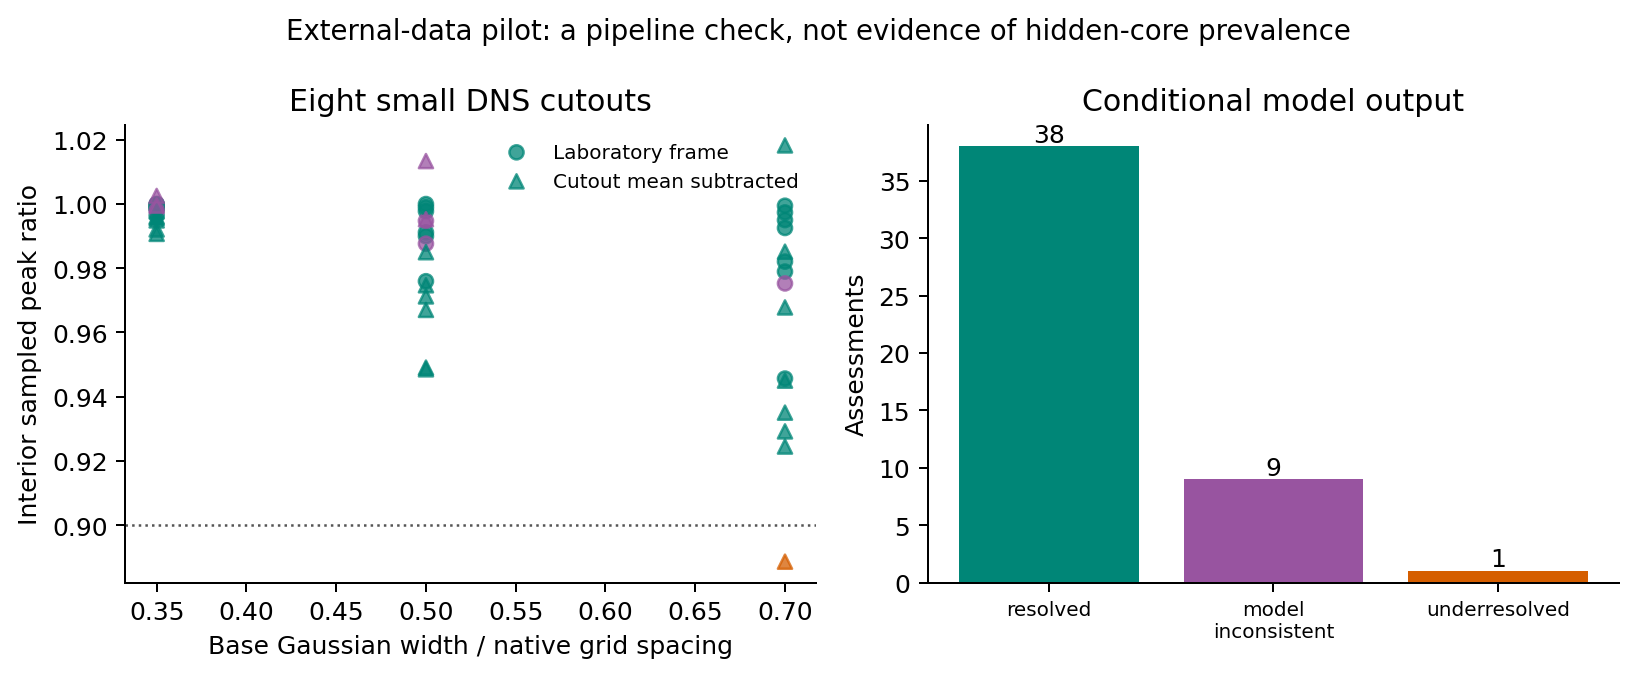
\includegraphics{figures/05_dns_pilot.png}
\caption{Small external DNS pilot. Colors identify conditional model
outcomes. The measured ratio uses a fixed interior grid region; it is
not a continuum retention certificate.}
\end{figure}

\textbf{Wider-filter follow-up.} One public 64\^{}3 JHTDB volume
{[}10{]} allowed widths 0.5, 1, 1.5, and 2 cells, evaluated on eight
nonoverlapping 16\^{}3 regions with 16-cell halos and two frame
conventions. A direct JHTDB query confirmed the mirror's 3\^{}3 prefix
exactly at float32 precision. Of 64 correlated assessments, 60 were
conditionally resolved, two underresolved, and two model inconsistent.
Fourteen resolved outputs had regional sampled ratios below 0.9. The
largest disagreement paired a conditional interval
{[}0.920798,0.921237{]} with a sampled ratio 0.684182. This is an
out-of-model disagreement, not a failure of the conditional theorem or
identification of a hidden core.

A post hoc field-of-view check used the full central 32\^{}3 region. One
of eight assessments still paired a resolved decision with a ratio below
0.9: {[}0.903977,0.904363{]} versus 0.880466. The reference maximum lay
on the region boundary in both frame conventions. Thus profile,
background, sampling, and field-of-view effects remain unresolved. These
experiments support caution about applying the model without its
hypotheses, but do not measure the prevalence of the analytic
hidden-core mechanism. The larger event-centered study in
\texttt{STUDY\_PROTOCOL.md} remains prospective.

\begin{figure}
\centering
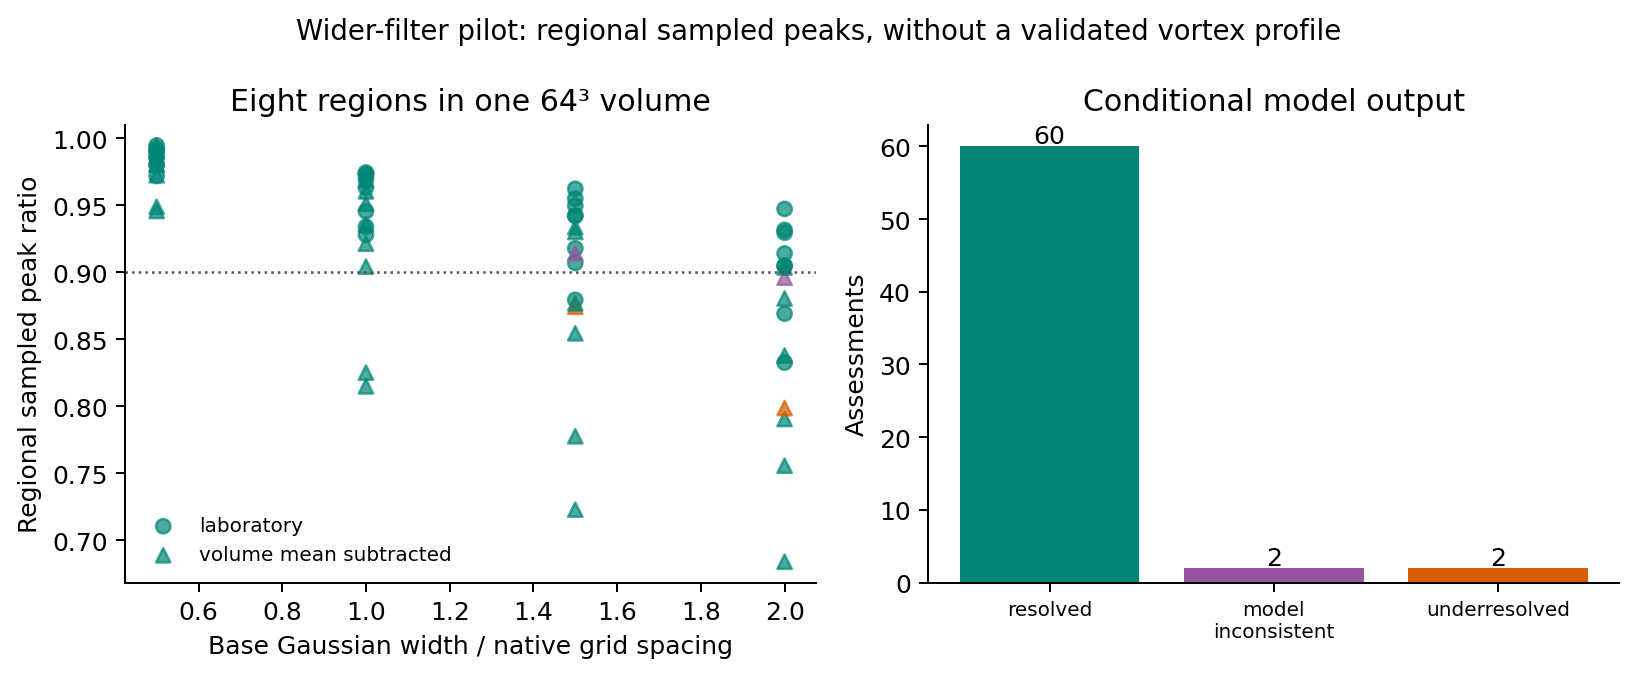
\includegraphics{figures/06_dns_extended.png}
\caption{Wider-filter pilot on eight regions in one public DNS volume.
Model decisions and regional sampled peak ratios can disagree; these
correlated assessments do not identify a physical hidden-core
mechanism.}
\end{figure}

\hypertarget{discussion-and-publication-scope}{%
\subsubsection{9. Discussion and publication
scope}\label{discussion-and-publication-scope}}

The main analytic result is the explicit nonuniform transition between
isotropic and anisotropic observation limits. The radial transfer has
power 3/2 and the axial transfer power 1/2 because the measured quantity
is the peak of a filtered vector vortex. This directional imbalance
creates the crossover in (13). It also permits separate recovery of the
two core scales from radial and axial changes in observation width.

The results give a precise meaning to apparent decay: a decreasing
measured peak can coincide with increasing true speed. A retention
interval is useful when the single-profile assumption is independently
justified. Without that assumption, the hidden-core example shows that
even extremely precise measurements and an excellent three-parameter fit
may leave most of the actual peak unresolved. Reporting the model
condition alongside a positive certificate is essential.

The completed internal review supports a narrowly framed technical note
containing an exact benchmark, a specific singular crossover, an
explicit model-failure example, and reproducible code. The basic
filtering and scale-selection mechanisms overlap established literature.
The 32/27 specialization alone does not justify a broad novelty claim.
Proposition 7 provides a limited connection to a full concentrating
flow; quantitative reconstruction of its filtered profiles remains a
separate problem. A stronger empirical or mathematical submission would
need new evidence about profile classes or actual measurements, beyond
the scope claimed here.

\hypertarget{reproducibility-authorship-and-status}{%
\subsubsection{Reproducibility, authorship and
status}\label{reproducibility-authorship-and-status}}

This manuscript and its calculations were developed with OpenAI Codex
assistance, including mathematical derivation, literature search, code
generation and execution, and manuscript preparation. Version 0.2
incorporated an internal audit of the proofs, arithmetic enclosures,
closest literature, and transfer claims, documented in
\texttt{REVIEW.md}. Version 0.3 adds an external DNS pilot and a
prospective validation protocol. No external referee or Lean
formalization was used. It is a public technical note with no claim of
established priority for the crossover. Code, editable sources, audit
data, and the manuscript are available in the
\href{https://github.com/Trenn1x/Trenn1x/tree/main/research/vortex-observability}{research
repository}. No journal acceptance or DOI is claimed. The work does not
assert a new Navier-Stokes blowup theorem.

\hypertarget{references}{%
\subsubsection{References}\label{references}}

{[}1{]} OpenAI. \emph{Finite time blowup for Navier-Stokes}. Released
September 2026. The source comparison used Sections 3 and 10 and
Proposition 9.9.
\href{https://cdn.openai.com/pdf/32d9f210-8b73-45e0-91bc-82a30aef8a9a/navier-stokes.pdf}{Manuscript}.
\href{https://openai.com/index/navier-stokes-solution/}{Announcement}.

{[}2{]} S. Rahgozar, Y. Maciel and P. Schlatter. Spatial resolution
analysis of planar PIV measurements to characterise vortices in
turbulent flows. \emph{Journal of Turbulence} 14(10), 37-66 (2013).
\href{https://doi.org/10.1080/14685248.2013.851386}{DOI:
10.1080/14685248.2013.851386}. Section 3.2.1 was checked in the
author-uploaded full text.

{[}3{]} E. Deem, A. Edstrand, R. Reger, K. Pascioni and L. Cattafesta.
Deconvolution correction for wandering in wingtip vortex flowfield data.
\emph{Journal of Fluid Science and Technology} 8(2), 219-232 (2013).
\href{https://doi.org/10.1299/jfst.8.219}{DOI: 10.1299/jfst.8.219}.

{[}4{]} T. Lindeberg. Principles for automatic scale selection. In
\emph{Handbook of Computer Vision and Applications}, volume 2, 239-274
(1999); KTH technical report (1998).
\href{https://www.csc.kth.se/cvap/abstracts/cvap222.html}{Author's
abstract and manuscript links}.

{[}5{]} T. Lindeberg. Discrete approximations of Gaussian smoothing and
Gaussian derivatives. arXiv:2311.11317 (2023).
\href{https://arxiv.org/abs/2311.11317}{Preprint}.

{[}6{]} T. Y. Hou. Blow-up or no blow-up? A unified computational and
analytic approach to 3D incompressible Euler and Navier-Stokes
equations. \emph{Acta Numerica} 18, 277-346 (2009).
\href{https://doi.org/10.1017/S0962492906420018}{DOI:
10.1017/S0962492906420018}.
\href{https://authors.library.caltech.edu/records/h8j4g-x8c18}{Author's
repository record}.

{[}7{]} L. Dong, W. Zhang, D. Xiao and X. Mao. Spatio-temporal
super-resolution reconstruction of particle image velocimetry-measured
vortex flows using generative adversarial networks. \emph{Journal of
Fluid Mechanics} 1022 (2025).
\href{https://doi.org/10.1017/jfm.2025.10775}{DOI:
10.1017/jfm.2025.10775}.

{[}8{]} T. Lindeberg. Scale selection properties of generalized
scale-space interest point detectors. \emph{Journal of Mathematical
Imaging and Vision} 46, 177-210 (2013); published online 20 September
2012.
\href{https://link.springer.com/article/10.1007/s10851-012-0378-3}{DOI:
10.1007/s10851-012-0378-3}. Full-text Sections 3.3 and 5.2 were checked.

{[}9{]} Johns Hopkins Turbulence Database. Forced isotropic turbulence,
isotropic1024coarse.
\href{https://turbulence.idies.jhu.edu/datasets/homogeneousTurbulence/isotropic}{Dataset
description}. \href{https://turbulence.idies.jhu.edu/database}{Access
documentation}. Downloaded 9 September 2026; exact indices and source
hashes are supplied in the release.

{[}10{]} ArielLubonja. Public JHTDB subset,
isotropic1024-coarse-velocity.h5.
\href{https://huggingface.co/datasets/ArielLubonja/johns-hopkins-turbulence-database}{Dataset
and source attribution}. Revision
9179e424e6eb75bcd89d3f608be795a633ccc1fa; native source consistency was
checked as described in the release.

\end{document}
